\providecommand{\FloatBarrier}{\clearpage}
\renewcommand{\topfraction}{0.92}
\renewcommand{\bottomfraction}{0.85}
\renewcommand{\textfraction}{0.06}
\renewcommand{\floatpagefraction}{0.75}
\setcounter{topnumber}{3}
\setcounter{bottomnumber}{2}
\setcounter{totalnumber}{5}


\section{Datasets}
\label{sec:data-methods}

Here we describe two principal datasets used in our analysis: Rubin Data Preview 2 catalogs and HST
data with star-galaxy labels used for testing methods discussed in \S 3. 


\subsection{Rubin Data Preview 2} 
\label{sec:data}

All data collected with the LSST Camera \cite{RTN-115} during the commissioning of the Rubin Observatory
will be released as Data Preview 2\footnote{See https://dp2.lsst.io/} (hereafter DP2). Coadded deep images and resulting catalogs have
been released in July 2026 as Early Data Preview 2. These coadded images are based on about 24,000
single-visit images and cover about 3,000 sq. deg. of sky. 

In our analysis we focus on the COSMOS field because it is both already well observed by Rubin (to
only about 1 magnitude shallower limit than anticipated for 10-year LSST), and space-based HST
COSMOS2020/FARMER star and galaxy labels are available \citep{2022ApJS..258...11W}. As a control
sample for testing code robustness, we also used Rubin data for the Extended Chandra Deep Field South (ECDFS). 
The Rubin $5-\sigma$ depth for point sources in the COSMOS field, estimated as the median magnitude
of point sources with photometric errors of $\sim$0.2 mag, is (25.66, 26.66, 26.36, 25.91, 24.94, 23.59)
in the $ugrizy$ bands, respectively. 


\subsection{HST Star-galaxy Classification Labels in the COSMOS Field} 

For the COSMOS validation sample, we select Rubin DP2 sources in the rectangular region
\(149.7 < {\rm RA} < 150.7\) and \(1.7 < {\rm Dec} < 2.7\), with
\(16 \le r_{\rm CModel} < 26\). Objects listed in the COSMOS2020/FARMER reference catalog are
matched to DP2 sources using a 0.5 arcsec matching radius. Within the selected region and magnitude
ranges, the DP2 sample contains 269,606 objects, of which 193,586 are matched to the
COSMOS2020/FARMER objects and 76,020 are unmatched (a matching fraction of 72\%). This
somewhat low matching fraction is due to large areas around bright stars that are masked in the
COSMOS2020/FARMER catalog (see Figure~\ref{fig:cosmos-footprint}). 

The matched validation sample contains 8,788 stars and 184,798 galaxies, classified using
HST's \(\texttt{truth\_binary}=1\) for stars and \(\texttt{truth\_binary}=0\) for galaxies. Their number
counts as function of magnitude are shown in Figure~\ref{fig:cosmos-magnitude-distribution}.
The low fraction stars is due to very faint sample limit $r \sim 26$) and high Galactic latitude ($b \sim
50^\circ$).  

\begin{figure*}[t]
  \centering
  
\includegraphics[width=0.9\textwidth]{fig01_cosmos_sky_coverage.png}
  \caption{
  The footprint for the DP2-COSMOS sample analyzed here. Gray points show Rubin DP2 objects 
  and  green points show the subset matched to the HST COSMOS2020/FARMER sample  
  a 0.5 arcsec matching radius. The white regions in the centers of gray areas correspond to
  areas where no objects are listed in either catalog. 
  }
  \label{fig:cosmos-footprint}
\end{figure*}

\begin{figure*}[t]
  \centering
  
\includegraphics[width=0.8\textwidth]{fig02_cosmos_dataset_overview.png}
  \caption{
  Magnitude distribution of the DP2-COSMOS sample. The black curve shows
  all selected DP2 sources, while the blue and red curves show matched
  COSMOS2020/FARMER sources classified as stars and galaxies, respectively.
  Counts are shown per magnitude, using 0.5 mag wide bins.  Note that galaxies
  outnumber stars at the faint end by more than an order of magnitude. 
  }
  \label{fig:cosmos-magnitude-distribution}
\end{figure*}



\subsection{The color-magnitude distributions of sources classified using HST labels}
\label{sec:reference-distributions}

The external COSMOS2020/FARMER labels provide the reference classification, considered here as ground
truth, for examining the distribution of stars and galaxies in various diagrams and for measuring
the performance of star-galaxy separation methods. Nevertheless, it is likely that some very faint
sources classified by HST as stars might be unresolved galaxies even at HST's resolution. Therefore,
the HST labels will help us assess whether a source should be resolved or unresolved in Rubin
images, but do not necessarily provide definitive information about astrophysical nature of a source
(e.g., to separate unresolved stars and galaxies, one would need spectra or broad-band photometry
over a much wider weavelength range, say, in near-infrared $K$ band). Furthermore, no classification
is perfect and thus we first examine the distribution of HST-classified ``stars`` and ``galaxies`` in
various informative color-color diagrams constructed with Rubin photometry. 

The top left panel in Figure~\ref{fig:truth_morphology_color} shows the distribution of stars and galaxies classified
using HST labels in the \(\Delta m = m_{\mathrm{PSF}} - m_{\mathrm{CModel}}\) vs. \(m_{\mathrm{CModel}}\)
diagram. As we describe in detail in the next Section, modeling this distribution is a key ingredient of the
Bayesian star-galaxy separation method presented here. 


The top right panel in Figure~\ref{fig:truth_morphology_color} shows that faint galaxies ($r>24$),
in addition to outnumbering stars at faint magnitudes, have on average bluer $g-i$ colors than stars. 
The clearly different distributions of stars and galaxies in color-color diagrams shown in the bottom
two panels in Figure~\ref{fig:truth_morphology_color}
demonstrate that colors can be used to enhance morphological star-galaxy separation. 
Nevertheless, Figure~\ref{fig:truth_color_color} and the top left panel in
Figure~\ref{fig:truth_morphology_color} clearly show that increased photometric noise close to the faint
magnitude limit will cause deteriorated performance for both morphological and color-based
star-galaxy separation methods. Extending the start of this deterioration to a fainter magnitude
limit is one of the primary goals of this work.  It is notable that the top right panel in Figure~\ref{fig:truth_color_color} 
implies that most unresolved faint blue sources have $u-g$ color more typical of low-redshift
quasars than of main sequence stars (for a detailed discussion of the blue star counts see
\citealt{2026A&A...707A.333P}). 


\begin{figure*}
  \centering
  
\includegraphics[width=\textwidth]{fig03_truth_morphology_color.png}
  \caption{The distribution of stars (blue dots) and galaxies (red countours), classified using HST labels, in various infomative
    diagrams. The CModel-magnitude based colors are corrected for the ISM dust extinction, while the $r$-band CModel magnitude is not.
   The top left panel shows the \(\Delta m = m_{\mathrm{PSF}} - m_{\mathrm{CModel}}\) vs. \(m_{\mathrm{CModel}}\) diagram, where
   stars form a narrow sequence centered on \(\Delta m \approx 0\) and for galaxies \(\Delta m >  0 \).  
   The top right panel shows the $r$ vs. $g-i$ color magnitude diagram and two bottom panels show
   most informative color-color diagrams. The main stellar locus, dominated by main sequence stars
   and red giants, is clearly visible with its blue end redwards from $u-g \sim 0.6$; unresolved sources with $u-g < 0.6$ are expected to be a
   mixture of low-redshift quasars, white dwarfs and unresolved binaries.}
  \label{fig:truth_morphology_color}
\end{figure*}


\begin{figure*}
  \centering
  
\includegraphics[width=0.8\textwidth]{fig04_truth_color_color.png}
  \caption{Similar to the bottom two panels in Figure~\ref{fig:truth_morphology_color}, except that
   here all principal color-color diagrams are shown and the data are split by the $r$-band CModel magnitude
   to show deterioration of photometry close to the faint magnitude limit (left: 16 $<$ rmag $<$ 25; right: 25 $<$
   rmag $<$ 26). The $5-\sigma$ depth for point sources in the $r$ band for this dataset is 26.36.}
  \label{fig:truth_color_color}
\end{figure*}

 

\subsection{The color-magnitude distributions of sources classified using \texttt{extendedness} parameter} 
\label{sec:extendedness-baseline}

Difficulties with star-galaxy separation encountered at the faint end are illustrated in
Figure~\ref{fig:r_extendedness_confusion_cmd}, which compares subsamples classified
using HST ground-truth labels and the default Rubin \texttt{extendedness} binary class in the $r$ band.
As evident, a significant fraction of faint sources within about two magnitudes from the faint limit are 
misclassified when using default \texttt{extendedness} parameter. Misclassifications have
a more severe impact on stellar sample: only 26\% of ``stars'' selected by \texttt{extendedness}=1
condition are unresolved in HST data. This high level of stellar sample contamination by faint
galaxies increases towards the faint end (see the bottom left panel in
Figure~\ref{fig:r_extendedness_confusion_cmd}).
As the same time, the selection completeness for ``stars'' (objects unresolved by HST) is only 67\%.
Due to much higher counts at faint magnitudes and high Galactic latitudes, the purity and
completeness for galaxies are much higher: 98\% and 89\%, respectively. In other words,
a simple classifier that declares every object to be a galaxy would formally perform quite well. 
Therefore, we will focus our analysis in the next Section on the classifier's performance when
selecting unresolved objects. 

\begin{figure*}
  \centering
  
\includegraphics[width=\textwidth]{fig05_r_extendedness_confusion_cmd.png}
  \caption{Performance of Rubin's default \texttt{extendedness} parameter in the $r$ band
    relative to HST ground-truth labels. The top left and bottom right panels show
    correctly classified unresolved and resolved sources in the $r$ vs. $g-i$ color-magnitude
    diagram, with counts shown in the title above each panel. The bottom left and the top right panels
    show misclassified sources. Note that the stellar sample selected by \texttt{extendedness}=0
    is severely contaminated by galaxies for \(r_{\mathrm{CModel}} > 24\) (bottom left panel).}
  \label{fig:r_extendedness_confusion_cmd}
\end{figure*}



\subsection{Suspect HST Classification Labels} 
\label{sec:suspectHST}


There is a subset of objects classified as ``stars'' (unresolved) by HST which appear clearly
resolved when using Rubin's default \texttt{extendedness} parameter. Figure~\ref{fig:suspectHSTccd}
shows their distribution in color-color diagrams, with symbols color-coded by \(\Delta m \) in the
$r$ band. As evident, their color-color distribution is inconsistent with main stellar locus and similar
to that expected for barely resolved or unresolved binary stars (see Figures 2 and 4 in \citealt{2004ApJ...615L.141S}.)
To test this hypothesis, we visually inspected several hundred images (443 objects with HST label
``star'', $r<23$ and $\Delta m > 0.05$ mag; see Figure~\ref{fig:suspectHSTimages} for an example). 
Only 1.4\% of selected objects are detected as ``isolated'' (computed using processing flag
``detect\_isIsolated'') and about half seem to have a nearby stellar-like companion. In some cases a
bright source or an extended galaxy is nearby, and about one tenth or fewer appear bluish and
consistent with quasars. Detailed examination of such cases is beyond the scope of this work. 

Because we aim to test statistical performance of our star-galaxy separation method on unambiguous
objects, we exclude objects with HST ``star'' label that both appear resolved in Rubin data and also
have Rubin colors inconsistent with the main stellar locus. 

{\bf DANIEL:} can you please add a paragraph here about how you rejected some HST stars by colors
and what were the numbers (fractions) of rejected objects (and how you handled variation with
magnitude)?  


\begin{figure*}
  \centering
  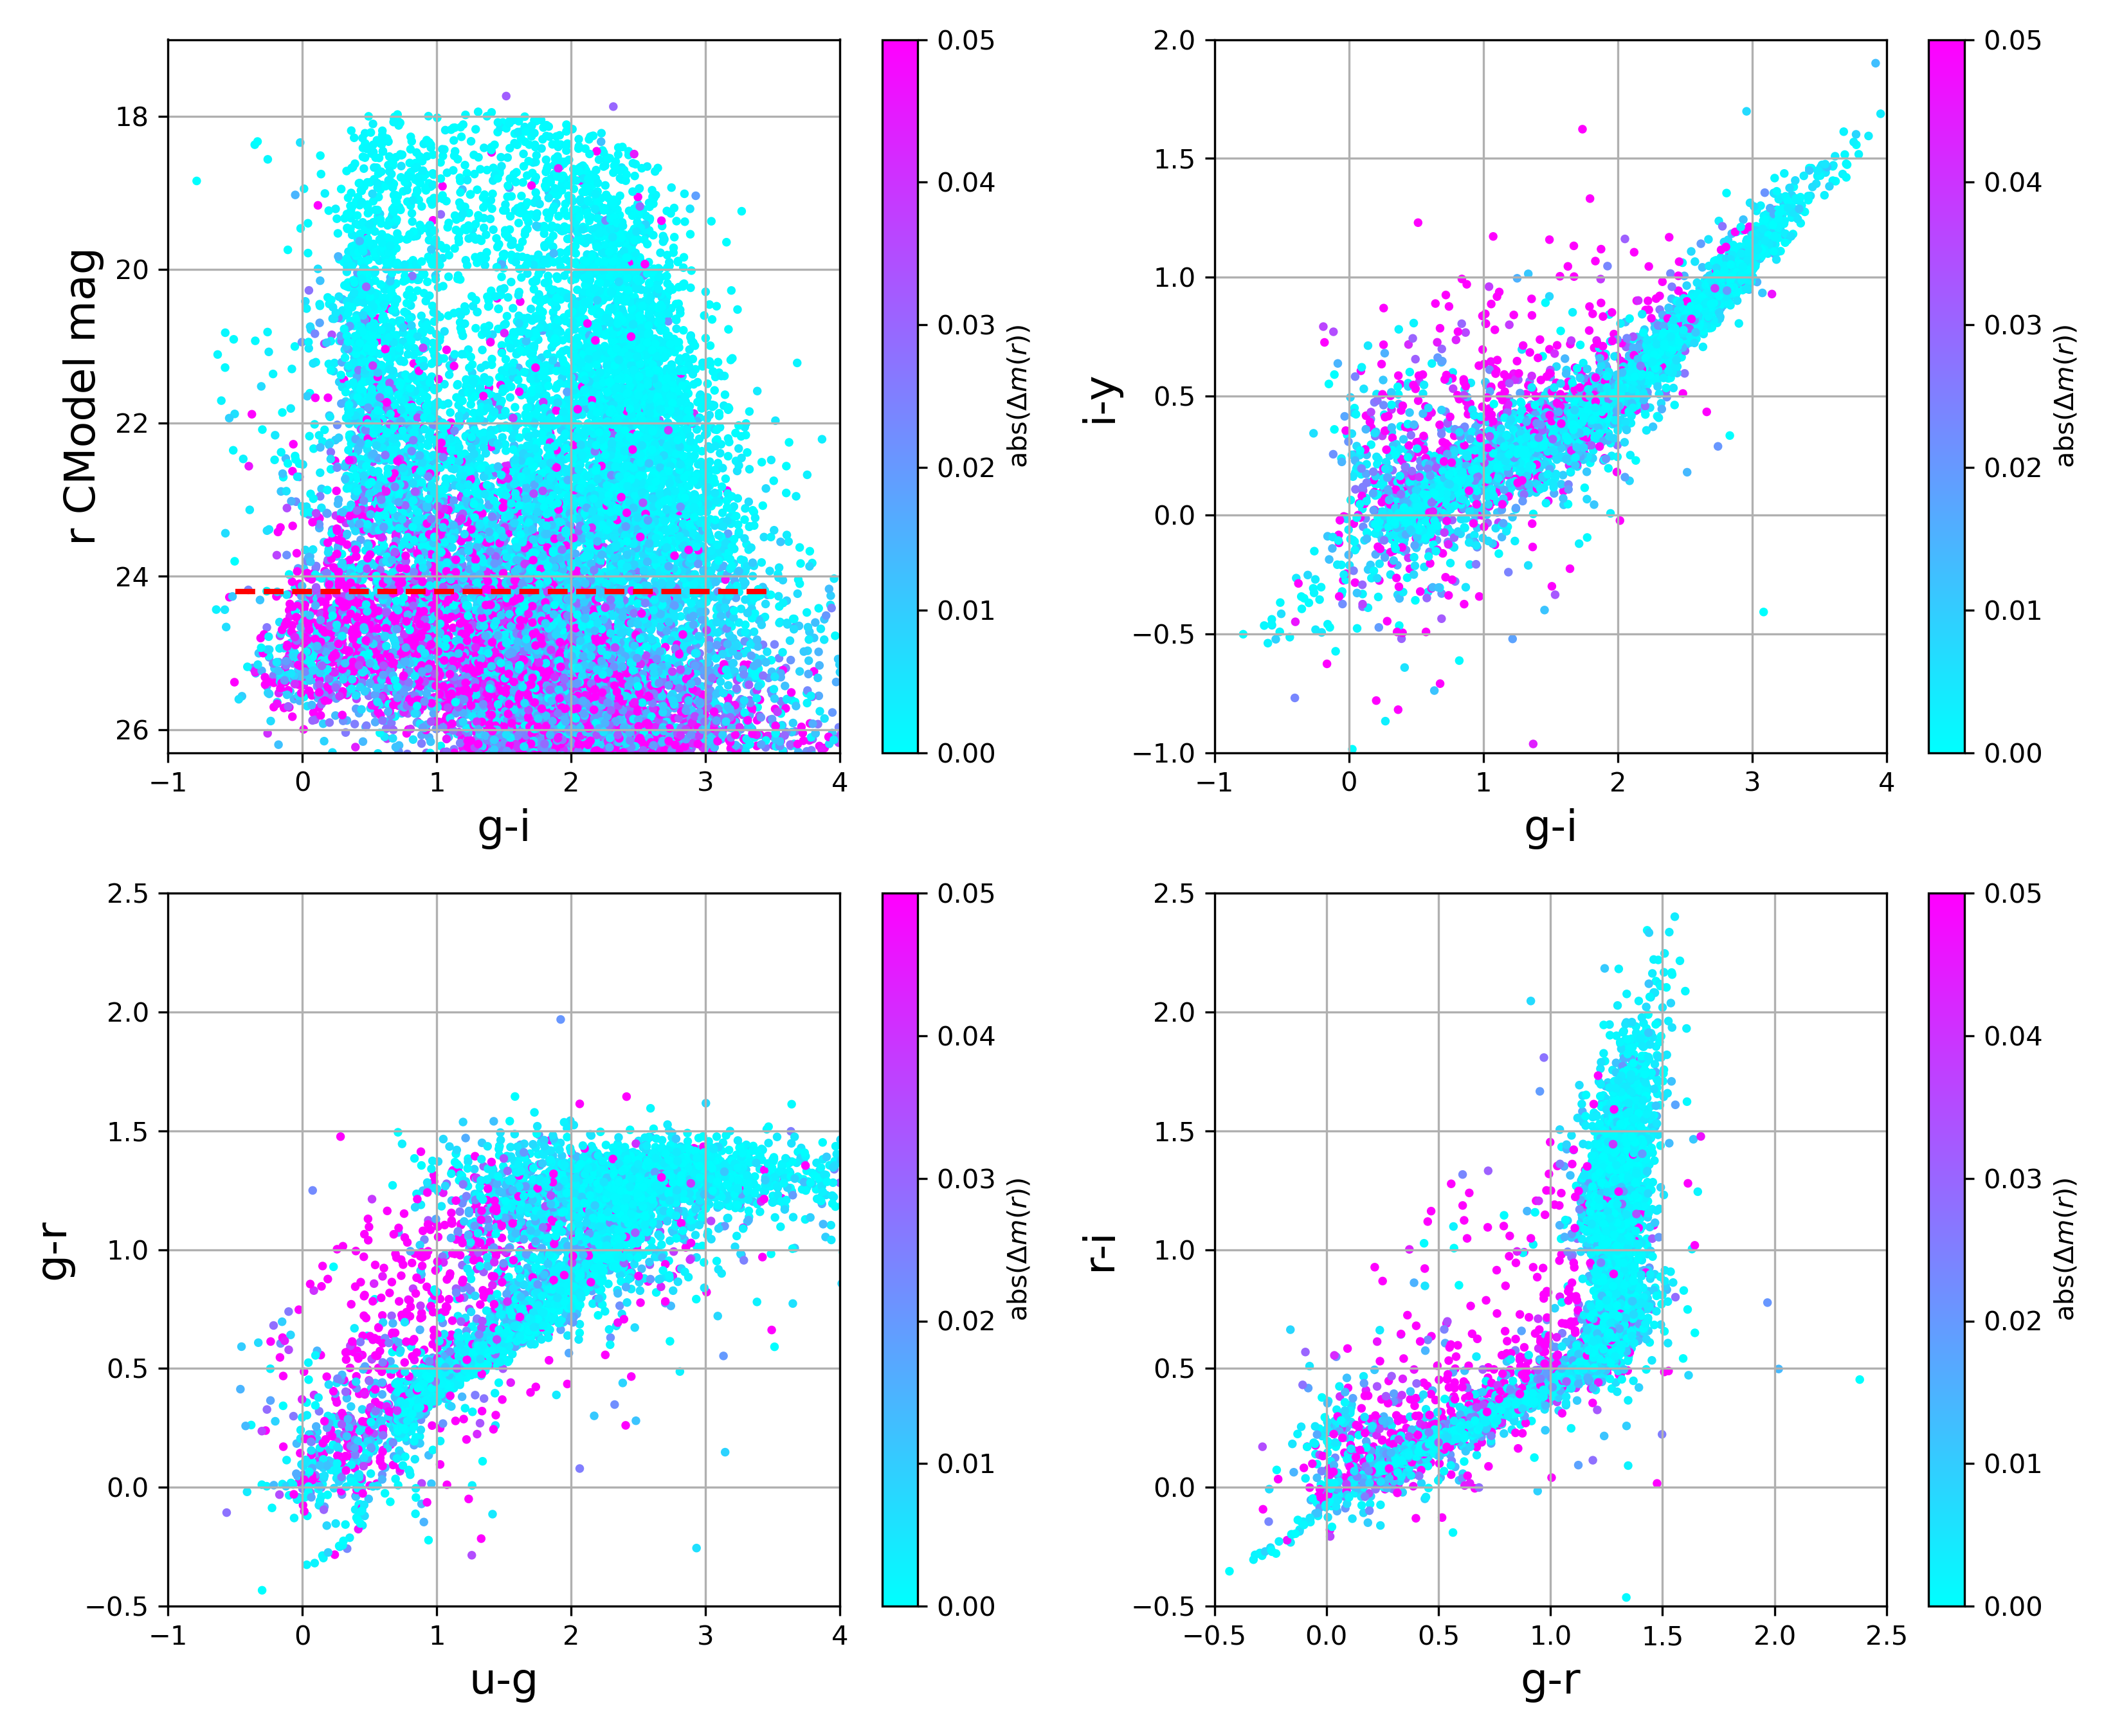
\includegraphics[width=0.9\textwidth]{COSMOSdm_HSTstarColored.png}
  \caption{The distribution of objects classified as ``stars'' by HST, but which appear clearly
    resolved when using Rubin's default \texttt{extendedness} parameter, in color-magnitude
    (top left) and informative color-color diagrams. Only objects with $r < 24.2$ are shown
    in the three color-color diagrams. Symbols are color-coded by the absolute value of
    Rubin's \(\Delta m \) in the $r$ band.  The color-color distribution of objects with
    $|\Delta m| > 0.05$ mag (about 3\% of all objects classified by HST as ``stars'' and brighter
    than $r=23$) is inconsistent with main stellar locus and similar to that expected for barely
    resolved or unresolved binary stars. 
}
  \label{fig:suspectHSTccd}
\end{figure*}



\begin{figure*}
  \centering
  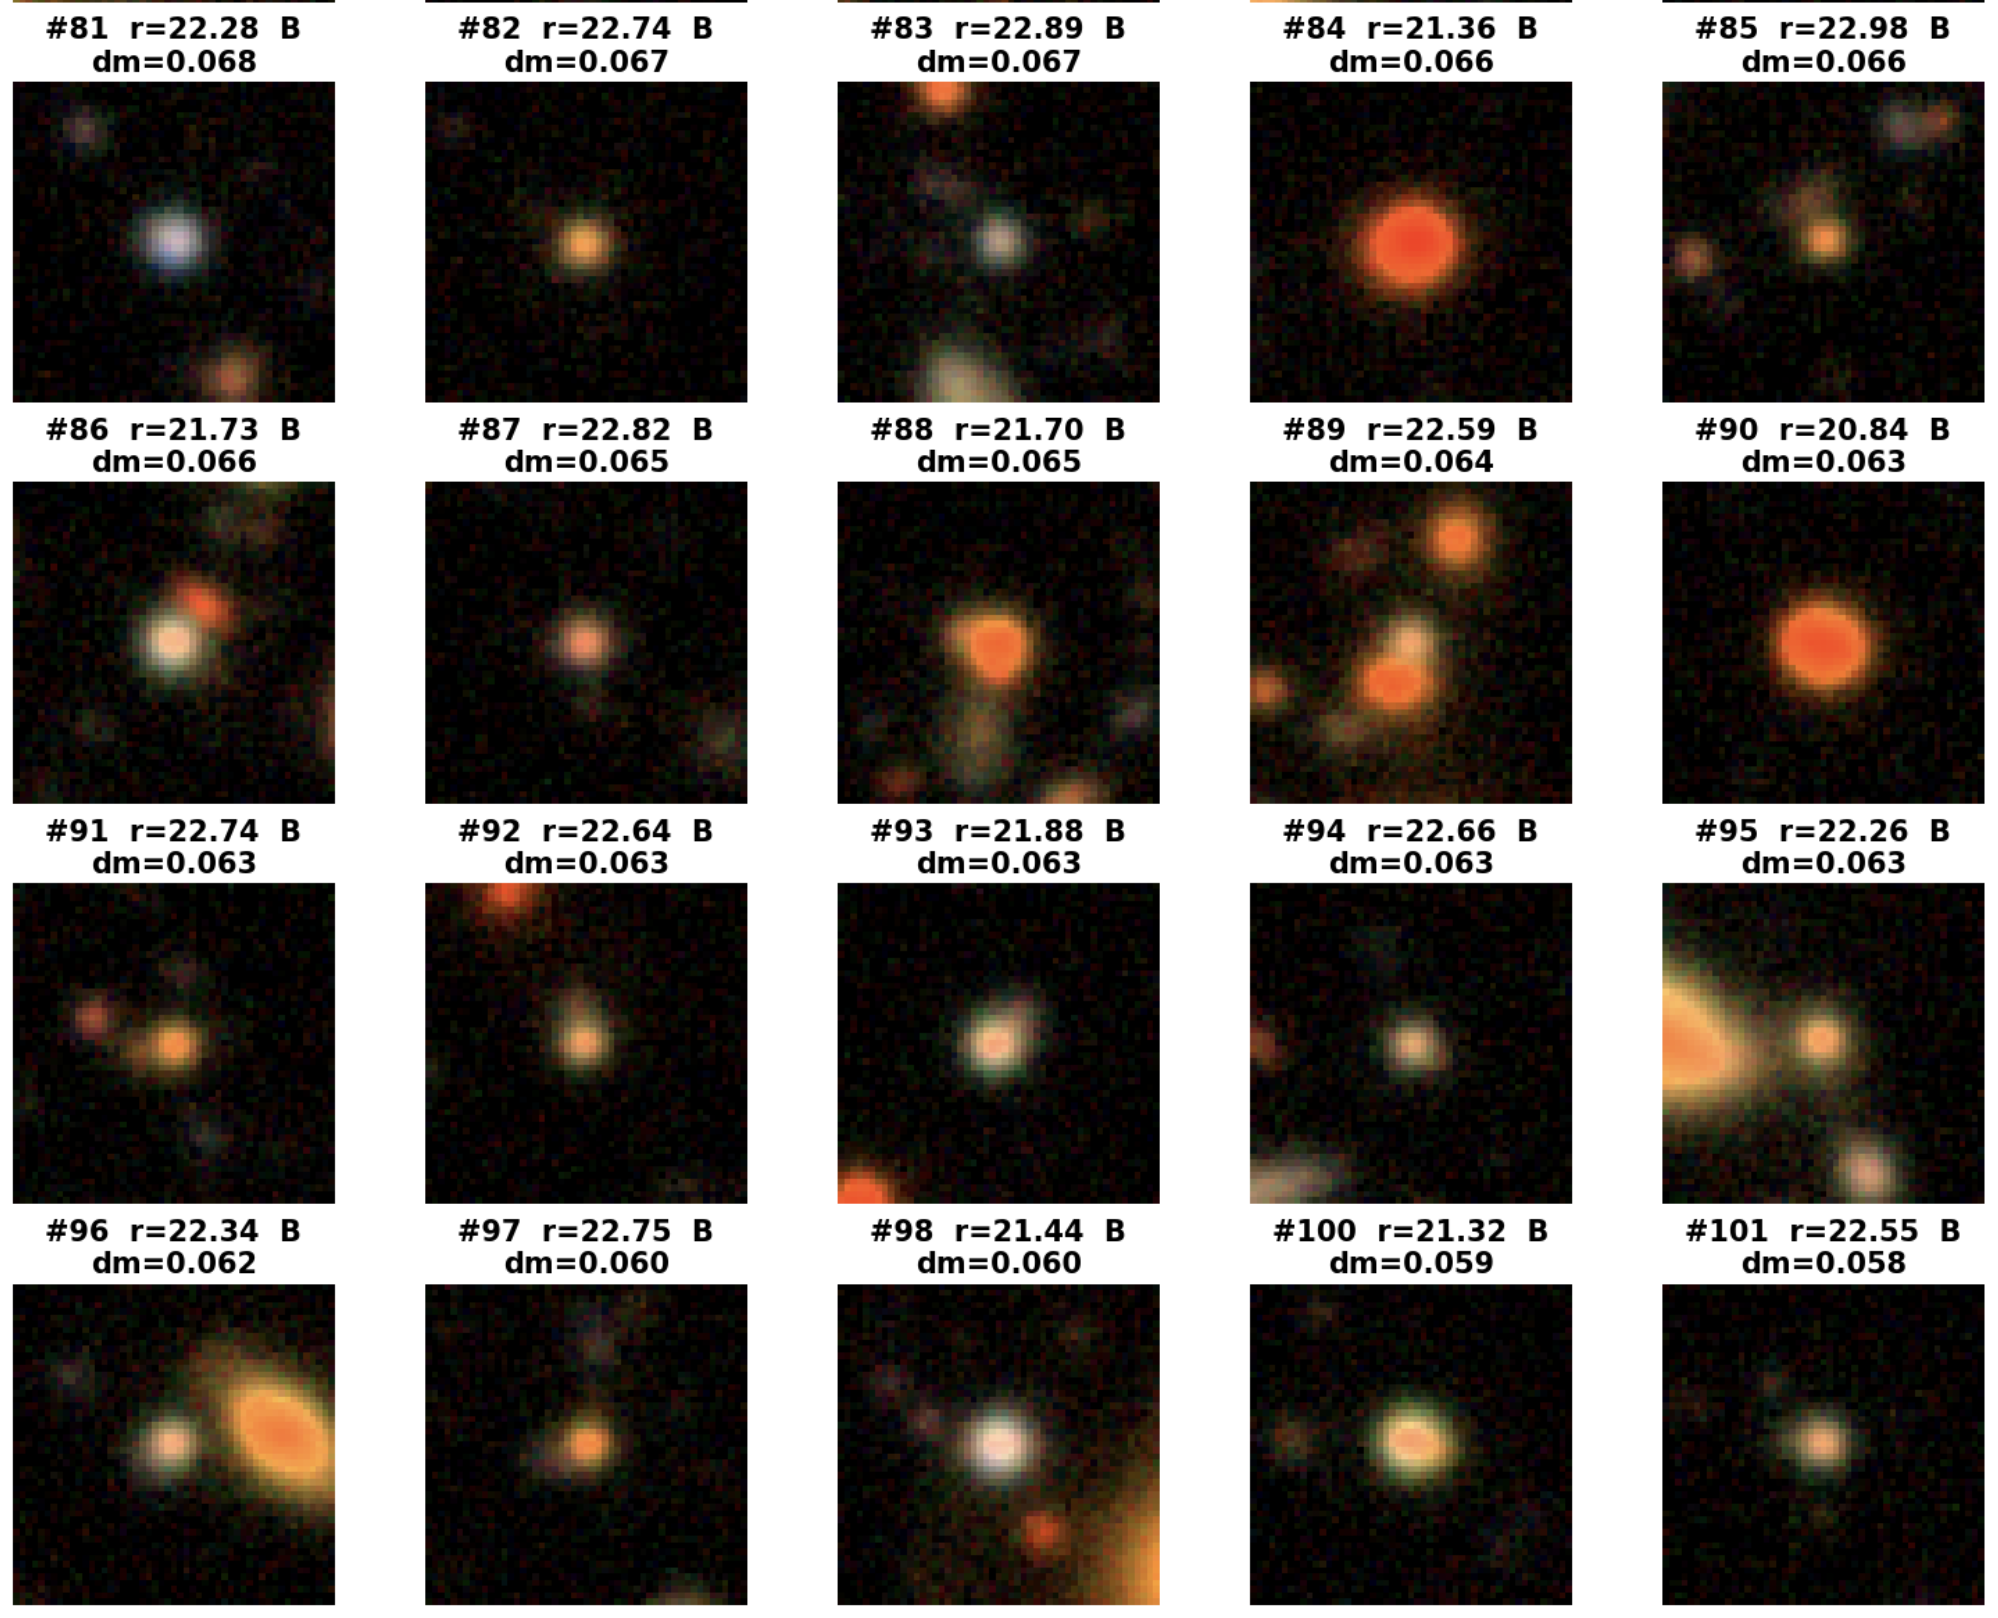
\includegraphics[width=\textwidth]{suspectHSTimages.png}
  \caption{The Rubin $gri$ color composite images extracted from ``deep\_coadd'', 10 arcsec by
    10 arcsec (50x50 pixels), for a random subsample of 443 objects selected as ``stars'' in HST and
    resolved in Rubin, and brighter than $r=23$. About 98.6\% are detected as blended objects.} 
  \label{fig:suspectHSTimages}
\end{figure*}
 